\documentclass[]{article}
\usepackage[hyphens]{url}
\usepackage[pdfusetitle,colorlinks,plainpages]{hyperref}
\usepackage[dutch]{babel}
\usepackage{lipsum} % for dummy text only
\usepackage{csquotes}
\usepackage[backend=bibtex]{biblatex}
%\usepackage[acronym]{glossaries}
\usepackage{eurosym}
\usepackage{subfigure}
\usepackage{multirow}
\usepackage{tikz}
\usepackage{listings}
\usepackage{caption}
\usepackage{pdfpages}

\usepackage{todonotes}
\usepackage{placeins}

\usepackage{tikz}
\usepackage{pgfplots}
\usepackage{verbatim}

%opening
\title{IMP: Pgpool-II}
\author{Thomas Uyttendaele}

\begin{document}

\maketitle
\section{Algemene inleiding}
In deze sectie zal voor de verschillende systemen de automatisering van installatie en configuratie met behulp van IMP uitgelegd worden. Er zal steeds de afhankelijkheden gegeven worden, een domeinmodel, uitleg bij het domeinmodel en voorbeeld configuratie gegeven worden. 

De automatisatie van installatie is ontwikkeld en getest met Fedora 18 en 20, op andere distributies en versies is er niet getest. 
Elk systeem maakt gebruik van \textit{ip::services::Server}, een instantie hiervan is een (virtuele) machine met een IP adres en besturingssysteem. 

Bij elke instantie is het verplicht om de firewall uit te zetten en SELinux op permissive te zetten. Dit kan met behulp van de volgende commando's: 
\begin{lstlisting}[frame=single, breaklines=true]
systemctl stop firewalld.service  
systemctl disable firewalld.service  
setenforce 0
sed -i "s/SELINUX=enforcing/SELINUX=permissive/g" /etc/sysconfig/selinux
sed -i "s/SELINUX=enforcing/SELINUX=permissive/g" /etc/selinux/config|
\end{lstlisting}

\section{Pgpool-II}
\textit{Link: \url{https://github.com/thuys/postgresql}}

Benodigde IMP modules: std, net, ip, redhat, hosts en yum. 

De installatie en configuratie is gebeurd aan de hand van de uitleg Pgpool-II\footnote{\url {http://pgpool.projects.pgfoundry.org/pgpool-II/doc/tutorial-en.html/}}. 

\subsection{Domein model en uitleg}
Het domeinmodel is te zien in figuur \ref{fig:imp-pgpool-domeinmodel}.

	\paragraph{PgpoolMain} Dit is de implementatie van de Pgpool-II router node. 
	
	\paragraph{PgpoolNode} Dit is de implementatie van de Pgpool-II data node die een uitbreiding is van de standaard PostgreSQL installatie. 
		
	\paragraph{PostgresqlServer} Dit is de implementatie van de standalone PostgreSQL server. 

\begin{figure}[ht!]
\centering
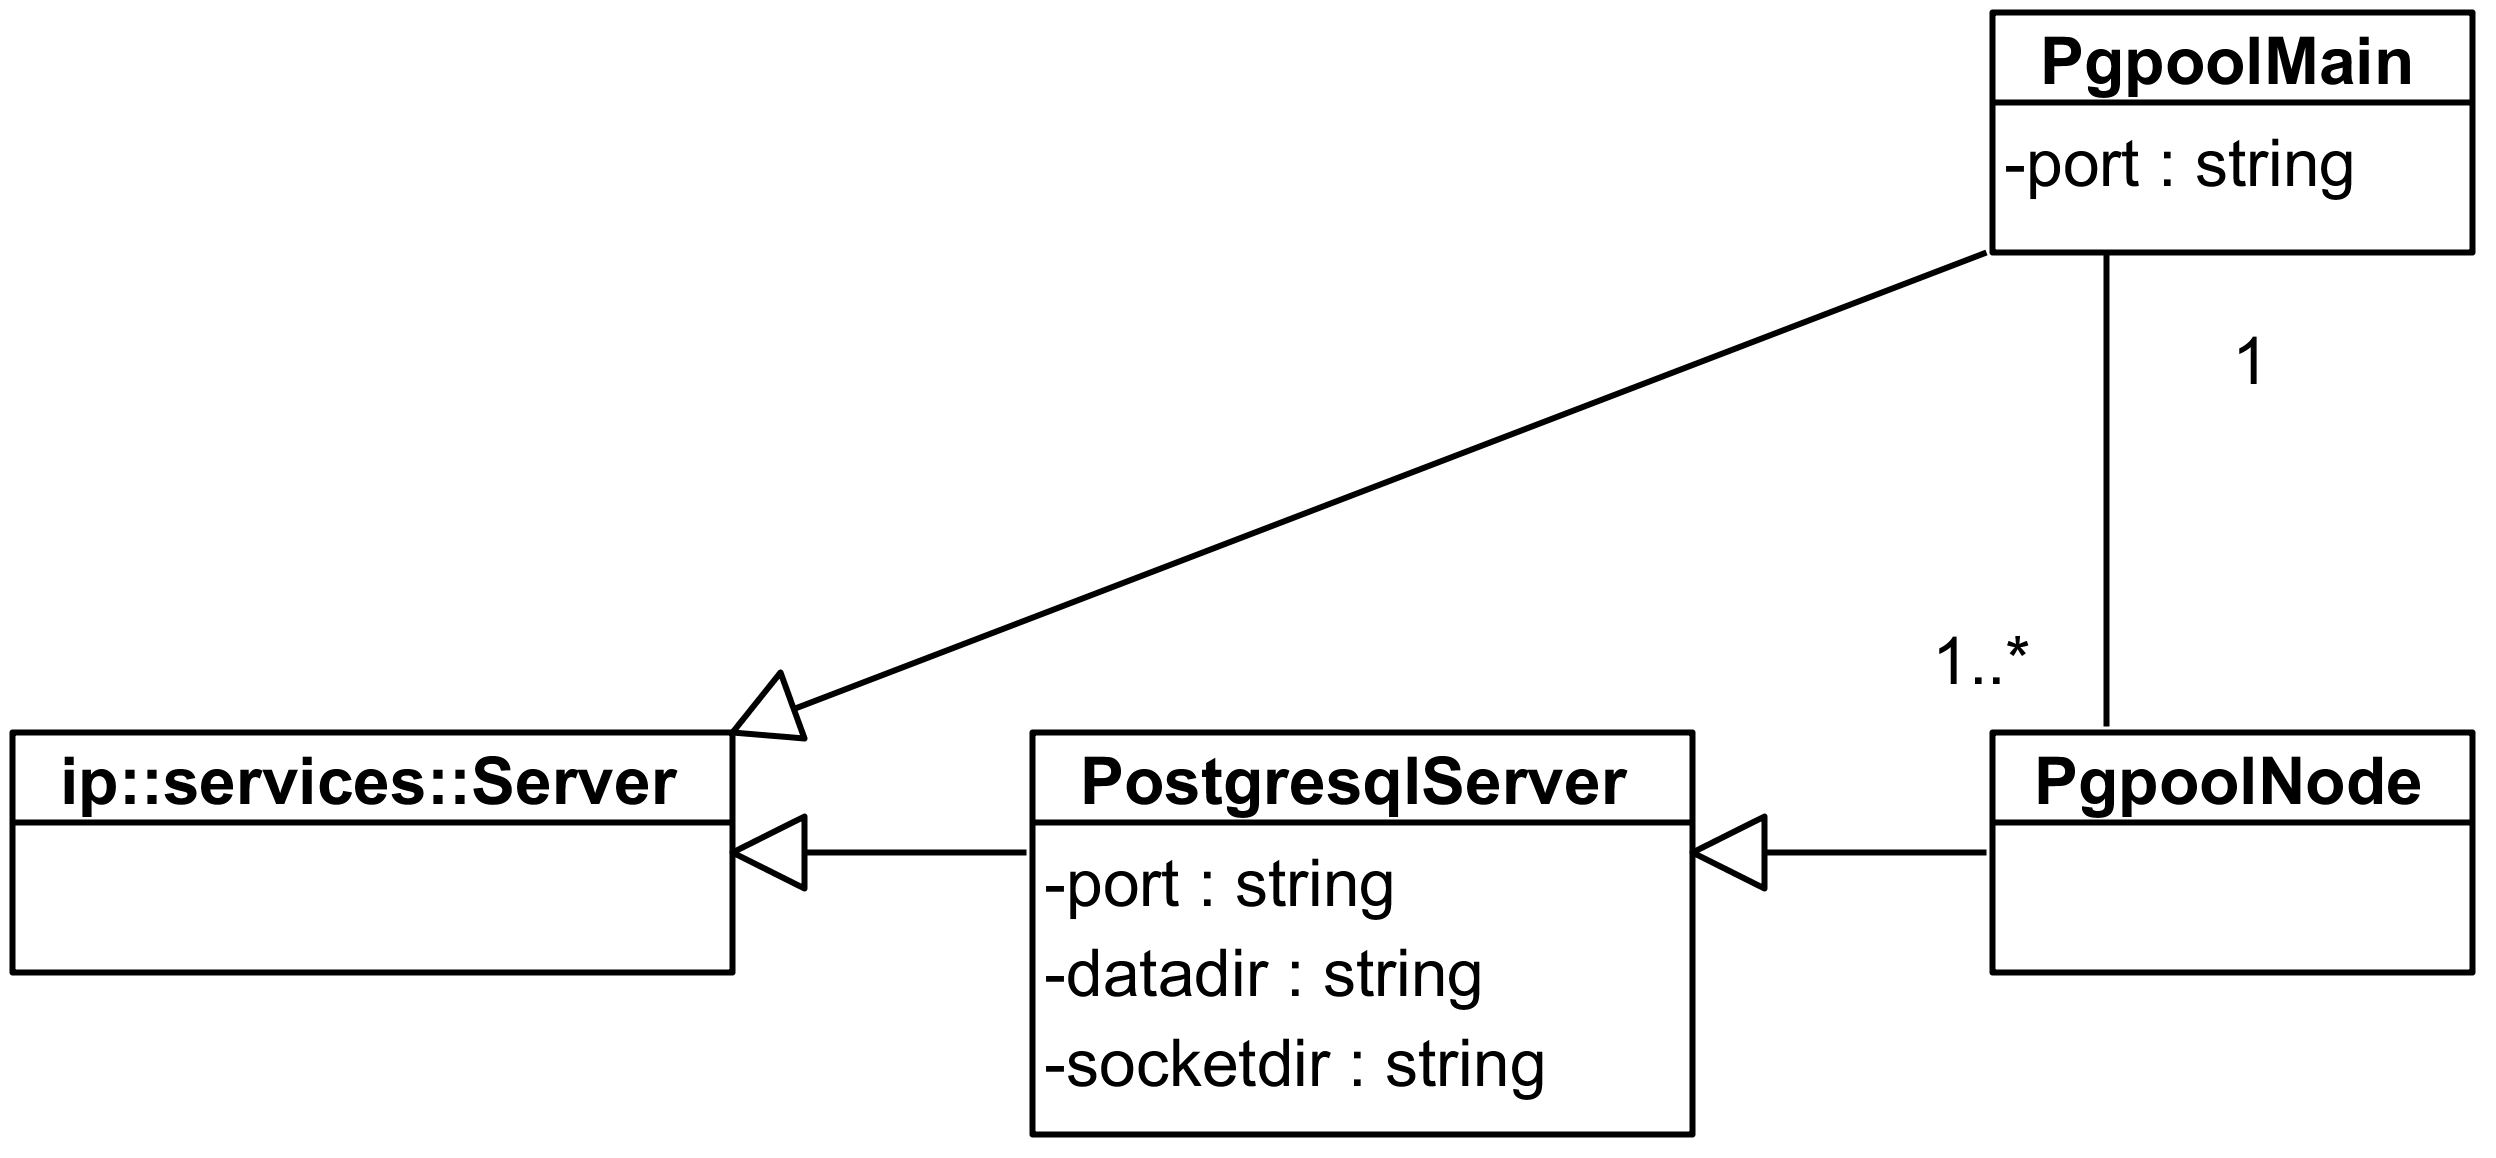
\includegraphics[width=\linewidth]{img/Postgres-Domeinmodel.png}
\caption{Pgpool-II: Domeinmodel Pgpool-II in IMP}
\label{fig:imp-pgpool-domeinmodel}
\end{figure}

\subsection{Voorbeeld configuratie}
De configuratie van Pgpool-II gebeurt in verschillende stappen: shell code, IMP uitrol, extra configuratie stap, IMP uitrol. 

De eerste shell code bestaat erin om de SELinux volledig uit te schakelen: 
\begin{lstlisting}[frame=single, breaklines=true]
systemctl stop firewalld.service  
systemctl disable firewalld.service  
echo "SELINUX=disabled SELINUXTYPE=targeted" > /etc/selinux/config

echo "SELINUX=disabled SELINUXTYPE=targeted" > /etc/sysconfig/selinux
\end{lstlisting}

De configuratie voor de testomgeving gaat als volgt in IMP: 

\lstinputlisting[language=Python, breaklines=true, frame=single]{code/imp-pgpool.conf}

De configuratie bestaat erin om al de verschillende nodes van Pgpool-II, ongeachte of dit routers of datanodes zijn, ssh toegang te geven tot elkaar server via ssh met root en postgres als gebruikers. Deze verbinding al een keer gemaakt zijn want een bericht dat de sleutel nu mee is opgeslagen is voldoende om de online recovery te doen falen. 

Hierna kan de IMP uitrol nog een keer gebeuren en het systeem zou moeten werken. 
\end{document}
